\documentclass{IEEEtran}
\usepackage[utf8]{inputenc}
\usepackage[T1]{fontenc}
\usepackage{natbib}
\usepackage{url}
\usepackage{hyperref}
\usepackage{amsmath}
\usepackage[pdftex]{graphicx}
% declare the path(s) where your graphic files are
\graphicspath{{images/}}
% and their extensions so you won't have to specify these with
% every instance of \includegraphics
\DeclareGraphicsExtensions{.pdf,.jpeg,.png,.jpg}

%allow more space between the words to prevent overfull boxes
\setlength{\emergencystretch}{1em}

\bibliographystyle{abbrvnat}
\setcitestyle{authoryear,round}

\title{Stock Prediction \\using Deep Learning and Google Trends Data}
\author{Michael Engel, Daniel Sikeler}
\date{\today}

\begin{document}
\maketitle
\renewcommand{\contentsname}{Table of Contents} 
\tableofcontents
\section*{Abstract}
\label{sec:abstract}
Irgendein Abstract... zusammenfassend vll.
\section{Introduction}
\label{sec:introduction}
Neural networks experienced a steep rise in popularity over the last years. One reason for this trend is the versatility of these networks. They are being deployed in many domains such as computer vision and pattern recognition, predictions, robotics and self-driving cars and many more. 
\\
However, quite few scientific papers of neural networks are released in the financial domain with the objective to predict the development of stock prices. The task of stock course prediction is difficult as the stock prices are influenced by a multitude of seemingly unpredictable and uncorrelated factors. Nevertheless, the development of a stock course depends strongly on the actions of traders. Those traders could use the search engine google to gather information about stocks they are interested in right before a trade. The service \textit{Google Trends} views various graphs displaying data of search terms typed in by users at the google search engine. This service is accessible by the public. Based on these thoughts the following hypothesis can be formulated: 
\\
\textit{A correlation between google trends search terms and stock courses exists. } 
\\
In this paper the previous hypothesis is being investigated. In order to check the existence of a correlation between goolge trends data and stock courses, a neural network will be implemented and verified. 
\section{Related Work}
\label{sec:relatedwork}
The stock market is commonly described as chaotic, volatile, complex and, therefore, seemingly unpredictable. However, the ability to predict the development of stock prices promises to yield much profit. Because of this there were many efforts to forecast the seemingly unpredictable. As a result of the hype for deep learning and its versatility of application, the scientific research to apply machine learning in the domain of stock market prediction was triggered. However, older scientific work does not provide encouraging results. Although this is rather unpromising, recent research work used the ever improving methods of deep learning to increase the precision of the forecast for stock development. 
\\
In \cite{stockprediction01}, for example, the authors propose a combination of (2D)2PCA and Deep Neural Network and compare the results with other state of the art methods. Compared to the 2-Directional 2-Dimensional Principal Component Analysis (2D)2PCA and Radial Basis Function Neural Network (RBFNN) the proposed method achieved an improved accuracy of 4.8\%. Also, the accuracy of the proposed DNN combination is about 15.6\% higher than the achieved precision of a Recurrent Neural Network (RNN). This result encourages the use of modern deep learning methods to predict stock development.
\\
A more comprehensive assessment was done in \cite{stockprediction02}. The authors analyzed advantages as well as drawbacks of different deep learning algorithms for predicting the stock development. They examined the fitness of three feature extraction methods, like the principal component analysis, on overall ability of the network to predict the development of the stock market. 
\\
In this paper a special form of RNN, the Long short-term memory network, is used to predict the future development of stock prices. Although the results in \cite{stockprediction01} discourage the use of RNN, the suitability of a LSTM was not investigated in the reference paper. Additionally, as the LSTM "remembers" values over an arbitrary interval of times, it is well-suited for predicting time series. By using Google Trends data as input it may prove as a valid model for predicting stock prices. The basic idea is described in more detail in \ref{sec:idea}. 
\section{Basic Idea}
\label{sec:idea}

google trends to stocks
simplified approach: only predict if the stock will increase or decrease
prediction of exact values are likely to have 0\% success rate

However, one key characteristic of stocks is that they are strongly volatile. 
Describe concept of volatility: (\url{https://de.wikipedia.org/wiki/Volatilit%C3%A4t})
absolute volatility:
\begin{equation}
	change = Value_{t1} - Value_{t0}
\end{equation}
relative volatility:
\begin{equation}
change = \frac{Value_{t1} - Value_{t0}}{Value_{t0}}
\end{equation}
logarithmic volatility:
\begin{equation}
change = ln(Value_{t1}) - ln(Value_{t0}) = ln(\frac{Value_{t1}}{Value_{t0}})
\end{equation}


in conclusion -> simplified approach reached xx\% of accuracy, therefore it would be worthwhile to enhance the current model by predicting ranges of values, e.g. 50 up or down etc.
as described in \ref{sec:architecture}, only minor changes would only be necessary
\section{Background}
\label{sec:background}
Deep learning architectures are complex and a lot of research is going on. In the next sections we provide some basic background knowledge about recurrent neural network. If further background knowledge about neural networks is necessary, please read \cite{DeepLearning}.

\subsection{Recurrent Neural Network}
\label{sec:rnn}
There are many architectures specialized on different tasks. Convolutional networks are used for processing data that is organized as grid, like images. This kind of nets can also be used for time-series data, which are a 1-D grid. But often the data can not be interpreted as a 1-D grid and then another architecture is better suited. Recurrent neural networks (RNN) are specialized on processing sequential data.\\
\begin{figure}[thb]
	\caption{recurrent neural network with hidden-to-hidden connections \cite[p. 373]{DeepLearning}}
	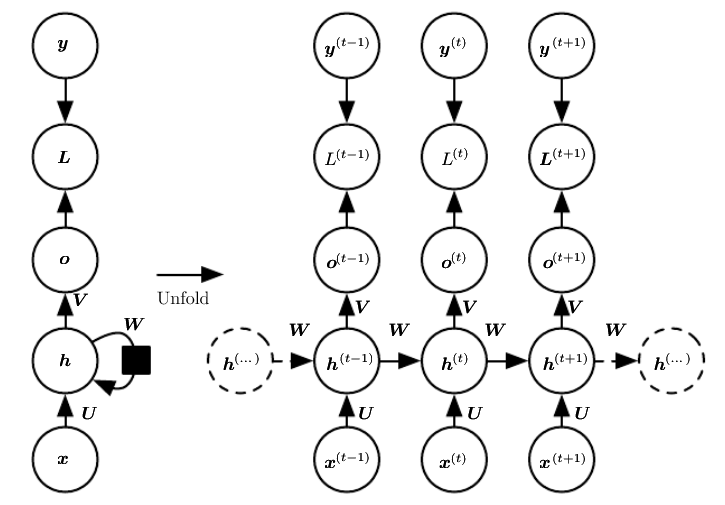
\includegraphics[width=0.95\linewidth]{images/rnn.PNG}
	\label{fig:rnn}
\end{figure}
The hidden units of a RNN have recurrent connections. So the result of a hidden unit at time step $t$ is used in the following time step $t+1$. It is important to notice that it is the same unit, which uses the result. As a consequence the parameters are shared during time. This is a key benefit, because it enables us to process sequences of different length. The update rule is also the same as it is the same unit.\\
There are different patterns, which combine the units in a different way. A RNN with connections between hidden units and a output at each time step (see figure \ref{fig:rnn}) can compute the same as a turing machine. In this sense the network is universal. It produces a sequence of outputs of the same length as the input. It is also possible to only produce a single output after the last hidden unit.\\
Like in any other neural network different output and loss functions are possible. Normally the softmax is used for the output. One common activation function is the hyperbolic tangent. The following equations show the update process of the forward propagation.
\begin{align}
a^{(t)} &= b + Wh^{(t-1)} + Ux^{(t)} \\
h^{(t)} &= tanh(a^{(t)}) \\
o^{(t)} &= c + Vh^{(t)} \\
y^{(t)} &= softmax(o^{(t)})
\end{align}
"where the parameters are the bias vectors b and c along with the weight matrices U, V and W, respectively, for input-to-hidden, hidden-to-output and hidden-to-hidden connections."\cite[p.374]{DeepLearning}\\
The generalized back-propagation algorithm can be applied to the unfolded computational graph. It is called back propagation through time (BPTT). You can see the unfold operation in figure \ref{fig:rnn}. Therefore, we need to store all the sequential states because they are used in the computation of the gradient. If we increase the number of recurrent layers the computational and memory cost increases as well. So for deep recurrent neural networks we have to meet the challenge of efficient training.

\subsection{Long-Term Dependencies}
\label{sec:ltd}
When we are training sequences of only length 10 to 20 the stochastic gradient descent (SGD) algorithm has already some problems. The gradients either tend to vanish, if it is in the interval $[0, 1[$, or tend to explode. The problem is that we reuse the unit in every time step and therefore the gradient is up to the power of the number of time steps.\\
Another problem is that the long-term dependencies have smaller magnitude on the weights than short-term dependencies have. The gradient is hidden by the smallest fluctuations arising from the short-term dependencies. As a consequence it takes very long time to train long-term dependencies. To overcome this problem we could introduce skipping connections where time step $t$ also uses the result from time step $t-2$ or even further in the past. So we have multiple time scales, one fine grained and one distant past.\\
Leaky units are a different way for remembering information about the past. A leaky unit is similar to a running average. A linear self-connection is used in the update rule.
\begin{align}
y^{(t)} = \alpha y^{(t-1)} + (1-\alpha)v^{(t)}
\end{align}
With the parameter $\alpha$ one could regulate how fast the information of the past is discarded. If $\alpha$ is near zero the information is kept for a long time. It would be the best if the network could learn this parameter and must not be set as a hyper parameter.

\subsection{Long Short-Term Memory}
\label{sec:lstm}
The Long Short-Term Memory (LSTM) is a gated recurrent neural network. Gated in this case means that the weight of the self-loop is controlled by another hidden unit. LTSM performed very good in handwriting and speech recognition, for example. The basic idea is that it might be useful to forget information of a leaky unit. As always it is better to have the network learn when to forget and not to decide manually.\\
\begin{figure}[thb]
	\caption{long short-term memory cell \cite[p. 405]{DeepLearning}}
	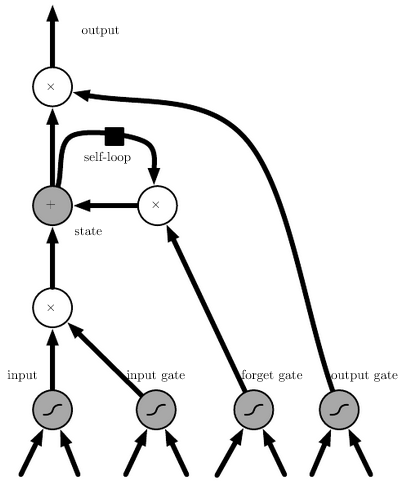
\includegraphics[width=0.95\linewidth]{images/lstmCell.PNG}
	\label{fig:lstm}
\end{figure}
In a LSTM network the hidden units consist of so called long short-term memory cells. A LSTM cell has three gating units (see figure \ref{fig:lstm}). The input gate is a sigmoid unit and controls the input feature. The input feature is a regular artificial neuron. The forget gate has the same task as the parameter $\alpha$ in a leaky unit. As there are only values between 0 and 1 are allowed, a sigmoid unit is used again. It controls how fast the information of the past is discarded. In other words it controls the weights of the state unit. The state unit has a self loop similar to the leaky units. With this self loop an internal recurrence is added to the outer recurrence of the LSTM cell. The output gate is also a sigmoid unit. It can shut off the output of the whole LSTM cell. So a Long Short-Term Memory network is far more complex than a simple recurrent neural network.

\subsection{Dropout}
\label{sec:dropout}

\section{Datasets}
\label{sec:datasets}
There are many databases, which provide a lot of datasets. One of those is \textit{kaggle}. \textit{kaggle} does not only provide datasets, they also organize competitions in analyzing datasets or improving already invented algorithms. We found a lot of data about to \textit{New York Stock Exchange}. Unfortunately we did not find one single dataset which satisfied all our requirements. There was no data about how often a search term was requested at \textit{Google}. So we had to collect the data ourselves from \textit{Google Trends}. In the following chapters we describe our datasets and why we are using them.

\subsection{Stock data}
We combined data about the \textit{New York Stock Exchange} of two datasets from \textit{kaggle}.
\label{subsec:stockdata}

\subsubsection{NYSE}
\label{subsub:nyse}
\cite{NYSE} collected information about historical prices of the S\&P 500 companies and additional fundamental data in his dataset. Standard and Poor`s 500 (S\&P 500) is a stock index of the 500 biggest US companies listed on the stock exchange.\\
The dataset has 4 files:
\begin{itemize}
	\item \textbf{prices.csv} This file contains the daily stock prices from 2010 until the end of 2016. For newer companies the range is shorter. Unfortunately the prices are sorted by day and not stock and therefore we could not use this data without preprocessing it. Instead, we found a better suiting dataset.
	\item \textbf{prices-split-adjusted.csv} Approximately 140 stock splits occurred during that time. This file has the same data with adjustments for the splits. We do not use this data neither.
	\item \textbf{fundamentals.csv} The file summarizes some metrics from the annual SECC 10K fillings. The metrics are useless for us, too.
	\item \textbf{securities.csv} Additional information for each stock can be found in this file. The most important data is the mapping from the ticker symbol to the full name of the companies. We use this data as an input for collecting data from \textit{Google Trends}.
\end{itemize}

\subsubsection{S\&P500}
\label{subsub:sp500}
The second dataset from \textit{kaggle} has also information about the daily stock prices from the S\&P 500. \cite{SP500} ordered the prices by stock and are therefore much more useful for us. Each entry consists of the date, four prices, the volume and its ticker symbol. The dataset has the prices for the last five years starting at 2012-08-13 until 2017-08-11. For the weekends there are no entries because the stock market is closed and no trading happens. For our task we use the opening and closing price to calculate if the stock went up or down on one day.


\subsection{Google Trends data}
\label{subsec:gtdata}
Google provides a public accessible service called Google Trends. It offers many different kinds of information about all search terms typed into the Google search engine. For example, for a given search term, like "Commerzbank", a graph is being displayed that shows the number of searches for this exact term over the course of time. The figure \ref{fig:gtexample} depicts a sample of this graph. 
\begin{figure}[!ht]
	\caption{Resulting graph of a google trends \cite{googletrends} search for the financial company "Commerzbank", which is tradeable at the stock market. }
	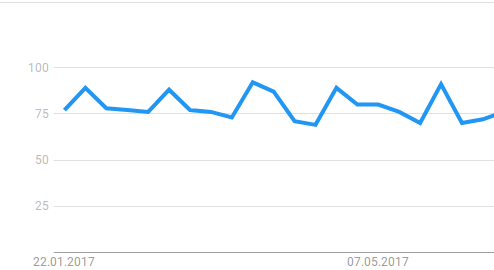
\includegraphics[width=0.95\linewidth]{images/googletrends.png}
	\label{fig:gtexample}
\end{figure}
Additionally, there is other data like the interest grouped by region, related topics and similar search terms available. Especially the similar search terms could be used to traverse all related Google Trends data starting from one single term like a stock course name. Therefore, the simple and automated extraction of Google Trend data is essential for the success of the proposed deep learning model for stock prediction. Unfortunately, there are some problems regarding the automated retrieval of it. This is explained in detail in the following subsection \ref{subsub:hackinggt}.

\subsubsection{Hacking Google Trends}
\label{subsub:hackinggt}
The amount of available data from Google Trends is massive. Unfortunately, unlike many other services of Google, it does not provide a public API for retrieving the trend data. Due to the needed quantity of data, manual extraction is not a practicable option. Therefore, an initial analysis of the sent requests from the web browser was executed. 
\\
The Google Trends website sends an explore-request to collect a JSON-file containing several tokens and further information. These tokens are used by the Google Trends servers to validate a request from the requesting machine to a specific service. The multiline-request is used to retrieve the time line data of a search term. The data for related topics and similar search terms can be collected by the same URL, whereas the respective token needs to be put as value into the token-parameter to distinguish between those two types of information. Based on this analysis, a python script is developed that gathers automatically the needed Google Trends data starting from the stock names. If too many requests are send to the server, the HTML error 429 may occur. This is being take care of by simply waiting a short period of time between the requests. 
\\
However, even the working python script was limited in a way that the Google Trend server only allows a limited number of requests. If that upper bound is reached, the server blocks the requests and redirects to another web address. On this website the user needs to prove that he is not a robot by clicking the parts of a picture that contain a certain object. Although the use of selenium, a framework to automate software tests for web applications, could serve as a possible workaround of this problem, it would imply a huge overhead with uncertain results. Therefore, this option was not further investigated. 
\\
The implemented python script for the automated Google Trend data retrieval, as well as the other related work of this paper, is published in the github repository of \cite{githubrepo}. 

\subsection{Merged dataset}
\label{subsec:merged}
From the three previously described datasets we used only two directly. The NYSE dataset (see \ref{subsub:nyse}) was only used to collect data from \textit{Google Trends} (see \ref{subsec:gtdata}). We combine the data of 14 search terms with the data from S\&P500 (see \ref{subsub:sp500}). We integrated the label in our dataset. The label is calculated from the opening and closing price.
\begin{equation}
y = sign(p_{close} - p_{open})
\end{equation}
The label can be found in the first column so that we can easily extract it in our algorithm. We separate our data in two classes. A label of $1$ means that the stock went up on this day. The other class is labeled with $-1$ and says that the price went down. If the value did not change during the day the label will be $0$. We interpret it the same as the label $-1$ because only up going prices are good if you invested in this stock.\\
The second column contains the opening price we already used to calculate the label. We did not include the closing value because it is the same as the opening price of the following day and could be computed. We include one price so that out network can use it to compare the trend of the stock price with the trends of the search terms. The value may be used to not only predict if the stock goes up or down, but to predict the exact next value.\\
The columns 3 to 16 contain the values of the search terms. It is important that there are only a few values of zeros. One problem is to find good search terms which are really correlated to the trend of the stock price. It is easily possible to replace them and test the network with other search terms. This may improve the prediction. We always include the search terms for the ticker symbol and the company name. The remaining twelve search terms depend on them.\\
Unfortunately it was not possible to collect data from \textit{Google Trends} for all search terms for the last five years. Therefore, we had to discard some of the stock prices and start including them in our dataset as soon as there are enough search terms with a different value than $0$. That is why the trends are starting at a different date.
The dataset can be preprocessed. Our preprocessing is described in the following chapter.
\section{Preprocessing}
\label{sec:preprocessing}
Because we use our own data set (created by our self), we do not need much preprocessing. We write the preprocessed data back to the file storage as python arrays (.nyp-files), so we do not have to do the preprocessing for each new training configuration. The csv-files contain the data as a two-dimensional array but we actually need a three-dimensional array. So we split the original data in blocks of dimension $30 \times 16$. If the number of entries in a csv-file could not be divided by 30 without remainder, the remaining entries are skipped.\\
For each block we apply zero-centering. Zero-centering is the method of subtracting the mean value of a column of each column entry. We do this only for the columns containing the data from \textit{Google Trends}. These values are all positive and therefore the gradient would also contain only positive or negative values, which makes training more difficult. We do not apply zero-centering to the opening price of the stock although we have the same problem with these values. But if we like to predict the new stock price and not only if the stock goes up or down, we need the original, unmodified price.\\
Another common preprocessing task is normalization. During normalization all values are mapped in a given interval. As the data from \textit{Google Trends} already is between $0$ and $100$ we do not need normalization. For the stock data we do it neither because of the same reason as before.\\
We have another preprocessing step which is not stored in the python array. The labels $-1$, $0$ and $1$ have to be converted in a array of dimension $1 \times 2$ as we only have to classes. The labels $-1$ and $0$ are treated as the same class. If the first entry of the array is bigger than the second, the stock price will rise. If it is the other way round the stock price will fall.
\section{Architecture}
\label{sec:architecture}

+ uml of project structure
+ describe every part of the uml and the connection between the parts
+ 
\section{Learning Model}
\label{sec:model}
The development of stock prices can be represented as a time series. The same applies to the Google trend data, where the number of searches for a specific term is used as y-value. These characteristics of both data types as well as the binary classification problem of predicting the rising or falling of the stocks urge the usage of a Long short-term memory network (LSTM). The necessary background for this type of network is explained in \ref{sec:lstm}. A common issue when training traditional RNN is the exploding and vanishing gradient problem. As LSTMs were developed to deal with those two problems, this advantage is another reason for using a LSTM. 
\\
As described in \ref{sec:architecture}, the model was separated in class. For higher flexibility an abstract base class \textit{LearningModel} was defined. Within this class the abstract function \textit{build\_graph} is declared. This method serves as the point of definition for the TensorFlow graph of the model. In \ref{subsec:simplelearningmodel} and \ref{subsec:onlystocklearningmodel} the implemented models used for stock prediction are explained. 

\subsection{Simple Learning Model}
\label{subsec:simplelearningmodel}
The \textit{SimpleLearningModel} class is derived from the abstract base class \textit{LearningModel} and, therefore, needs to implement the \textit{build\_graph} function. A initial check if the graph has already been built prevents a possible exception. The first action when defining the TensorFlow graph is the creation of variables for the input X and the labels Y. Consequent, the variables for the weights and bias are defined and randomly initialized. The \textit{SimpleLearningModel} uses just a single LSTM-cell with a configurable hidden size and forget bias. This simple model also facilitates the use of dropout. If dropout is specified, a \textit{DropoutWrapper} is wrapped around the created LSTM-cell with a fixed dropout rate. The softmax function is used to predict the direction of future stock prices:
\begin{align}
prediction &= softmax(input \cdot weights + bias)
\end{align}
The loss is calculated by applying the summary metric \textit{cross entropy} to the unscaled output. This metric was deployed, because the cross entropy should be optimally minimized and the softmax function is used for the prediction. Therefore, numerically unstable corner cases are covered in a mathematically suitable way. For optimization the \textit{GradientDescentOptimizer} is facilitated by the model. Although this simple Optimizer requires more tuning of the learning rate to converge quickly, it does far less computations than the \textit{AdamOptimizer}. For training the minimization operation is applied to the loss. 

\subsection{Only Stock Learning Model}
\label{subsec:onlystocklearningmodel}
In comparison to the \textit{SimpleLearningModel} the \textit{OnlyStockLearningModel} uses far less information. The whole data from \textit{Google Trends} is discarded during runtime. As the \textit{SimpleLearningModel} can be configured very easily, the \textit{OnlyStockLearningModel} is derived from it. The only adaption is that the number of values (columns) used from the dataset is fixed to only the column with the stock data.
\section{Evaluation}
\label{sec:evaluation}
For evaluation of both models, which are described in section \ref{sec:model}, the tool \textit{Tensorboard} is used. This suite of visualization tools can be used to understand, debug and optimize \textit{TensorFlow} programs. In the context of evaluation, \textit{Tensorboard} is used to visualize the 
\begin{itemize}
	\item accuracy,
	\item loss and
	\item graph
\end{itemize}
of the model. As validation technique the k fold cross validation is being deployed. How this technique works and how it is integrated within the architecture is described in the subsection \ref{subsec:kfoldxvalidation}. In \ref{subsec:experiments} the basic setup used for executing different experiments are explained. The specific results of those experiments for the \textit{SimpleLearningModel} are shown in subsection \ref{subsec:slmexperiment}, while the results yielded by the \textit{OnlyStockLearningModel} are described in the subsection \ref{subsec:onlystockmodelexperiment}. Finally, the results from both models are compared in subsection \ref{subsec:compmodelresults}.

\subsection{K fold cross validation}
\label{subsec:kfoldxvalidation}
The most simple method for cross validation is the \textit{holdout} method. This technique splits the available dataset into two distinct sets - training and validation. In terms of variance this method is disadvantageous as it is not certain which data points end up in the validation set. This can lead to losing important patterns during training and, therefore, underfitting. 
\\
The technique of k fold cross validation provides a method of using the available data efficiently for training as well as validation. The data is split into $k$ subsets and the \textit{holdout} method is applied $k$ times to these sets. In each iteration a different set of the $k$ datasets is used as validation set and the remaining $k-1$ sets are used for training. As a result, each data point is used multiple times for training at some point in the loop and once for validation. Consequently, most of the data is used for fitting so that the bias is greatly reduced and by using most data for validation this also reduces the variance. The swap of training and validation data for each iteration also contributes to the efficiency of this technique. 
\\
The evaluation of the model by the k fold cross validation is achieved by logging the accuracy and loss. Those two scalars are measured for every iteration during the cross validation and after the $k$ iterations for the current epoch. During each of the $k$ iterations the mean of the accuracy and loss for all batches is calculated and written to a \textit{Tensorboard} chart. After the $k$ iterations the mean of all previously calculated average accuracies and losses is determined and also written to a \textit{Tensorboard} chart, whereas the x-axis displays the epoch of this result. The calculation for those mean values is done outside the \textit{TensorFlow} graph. Although this is not best practice, the mean calculation for those scalars would have been quite challenging to do inside the graph as a definition for the epoch is not possible at the level of graph definition. 

\subsection{Experiments for evaluation}
\label{subsec:experiments}
For the validation of the model implementation experiments are executed for both defined models, which are described in detail in subsection \ref{subsec:simplelearningmodel} and \ref{subsec:onlystockmodelexperiment}. The following parameters are varied for a different setup: 
\begin{itemize}
	\item dropout probability, 
	\item hidden size of the LSTM cell, 
	\item learning rate of the optimizer, 
	\item count of folds for cross validation $k$, 
	\item and the number of epochs
\end{itemize}
The mean accuracy and loss after each k fold cross validation as well as the mean overall accuracy and loss are being used as metrics for the rating of parameter configuration. These scalars are logged as described in the previous subsection \ref{subsec:kfoldxvalidation}. 
\\
Overall, four different settings of those parameters are used, wherefore four experiments for each model type are executed. In table \ref{tbl:experiments} these configurations are depicted. 
\renewcommand{\arraystretch}{1.5}
\begin{table}[!ht]
	\begin{center}
		\begin{tabular}{c|c|c|c|c|}
			\multirow{2}{1cm}{} & \multicolumn{4}{c|}{\textbf{Experiment setups}} \\
			 & \textbf{1} & \textbf{2} & \textbf{3} & \textbf{4}\\
			\hline
			\textbf{Hidden size} & 100 &  100 & 200 & 100 \\
			\hline
			\textbf{Dropout probability} & 0.3 & 0.0 & 0.3 & 0.3 \\
			\hline
			\textbf{Learning rate} & 1.0 & 1.0 & 2.0 & 0.5 \\
			\hline
			\textbf{Number of folds k} & 10 & 10 & 10 & 10 \\
			\hline
			\textbf{Number of epochs} & 650 & 650 & 650 & 650 \\
		\end{tabular}
	\end{center}
	\caption{The configurations for all experiments. }
	\label{tbl:experiments}
\end{table}
While the number of folds k for the cross validation as well as the number of epochs for training remain the same for all experiments, the other three parameters are varied. According to a scientific paper about dropout from the university of Toronto (\cite{Srivastava:2014:DSW:2627435.2670313}) the minimal classification error is achieved for a fixed dropout probability $p$ in the range $0.3 \le p \le 0.8$. Therefore, the experiments using dropout are executed with a minimal dropout probability $p = 0.3$. To examine the effects of the hidden size of the LSTM cell and the learning rate of the optimizer on the accuracy and loss, these parameters are also varied. 
\\
Additionally, the trained model is used to predict the rising or falling of stocks unused during the training process. This prediction process is executed ten times and the maximum, minimum and average accuracy for the predictions are logged. Thus conclusions can be made about the applicability of the models for stock prediction. 

\subsection{SimpleLearningModel results}
\label{subsec:slmexperiment}	
The visualized experiment results of the \textit{SimpleLearningModel} are extracted from \textit{Tensorboard}. Within the visualization suite the accuracy and the loss of all experiments were grouped within one graph for better comparability. In figure \ref{fig:acc650epochs} the accuracy over 650 epochs are depicted. 
\begin{figure}[!ht]
	\caption{The mean accuracy of all experiments over 650 epochs of the k fold cross validation with $k=10$. }
	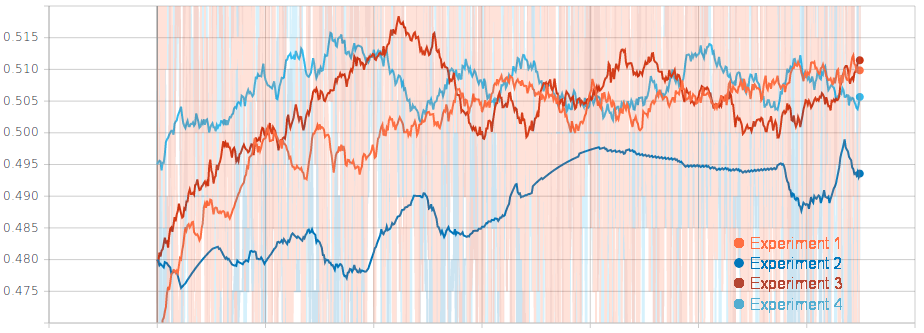
\includegraphics[width=0.95\linewidth]{images/evaluation/slm-k-accuracy.png}
	\label{fig:acc650epochs}
\end{figure}
\\ As expected, the experiment without dropout achieved the lowest accuracy of all experiments. While the other three experiments achieved quite similar results concerning the accuracy, experiment 2 needed about twice the time for the same number of epochs than experiment 1 and 4 with about 22 minutes. This is due to the doubled size of the hidden units, wherefore this setting is unsuitable for training and, also, strongly influences the extent of the loss which can be seen in figure \ref{fig:loss650epochs}. 
\begin{figure}[!ht]
	\caption{The mean loss of all experiments over 650 epochs of the k fold cross validation with $k=10$. }
	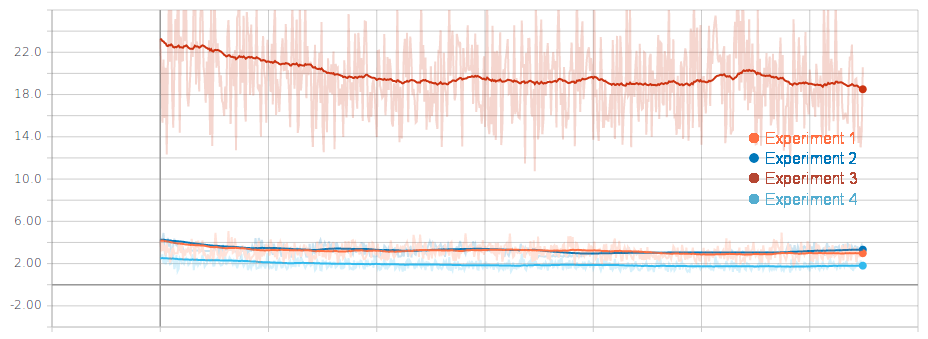
\includegraphics[width=0.95\linewidth]{images/evaluation/slm-k-losses.png}
	\label{fig:loss650epochs}
\end{figure}
\\ Therefore, only experiment 1 and 4 yield acceptable results. In comparison, the accuracy graph of experiment 4 is overall higher than the accuracy graph of experiment 1. This implies that the configuration of experiment 4 is better than the settings of experiment 1. However, regarding the prediction results for a dataset unknown to the trained models, experiment 1 seems to work better. In table \ref{tbl:slmpredictresults} these prediction results are presented. 
\begin{table}[!ht]
	\begin{center}
		\begin{tabular}{c|c|c|c|c|}
			\multirow{2}{1cm}{} & \multicolumn{4}{c|}{\textbf{Experiment setups}} \\
			& \textbf{1} & \textbf{2} & \textbf{3} & \textbf{4}\\
			\hline
			\textbf{Minimum} & 50.00 & 43.75 & 43.75 & 31.25 \\
			\hline
			\textbf{Maximum} & 68.75 & 43.75 & 68.75 & 68.75 \\
			\hline
			\textbf{Average} & 61.25 & 43.75 & 50.00 & 51.25 \\
		\end{tabular}
	\end{center}
	\caption{The minimum, maximum and average prediction accuracy in \% of ten predictions for a dataset unknown to the trained \textit{SimpleLearningModel}. }
	\label{tbl:slmpredictresults}
\end{table}
As described in the previous section \ref{subsec:experiments}, these results are collected by using a dataset unknown to the trained models and executing the prediction function ten times. For this validation the settings of experiment 1 achieve a 10\% higher accuracy than the model of experiment 4. The smaller learning rate of experiment 4 in combination with the presented results could imply that this model needs more epochs to converge to the optimum. However, the losses of all experiments quickly converge to a minimum. In figure \ref{fig:loss650epochs2} the graph of the third experiment is removed due to its magnitude so that a more precise view of the remaining loss graphs can be seen. 
\begin{figure}[!ht]
	\caption{The mean loss of the experiments 1, 2 and 4 over 650 epochs of the k fold cross validation with $k=10$. }
	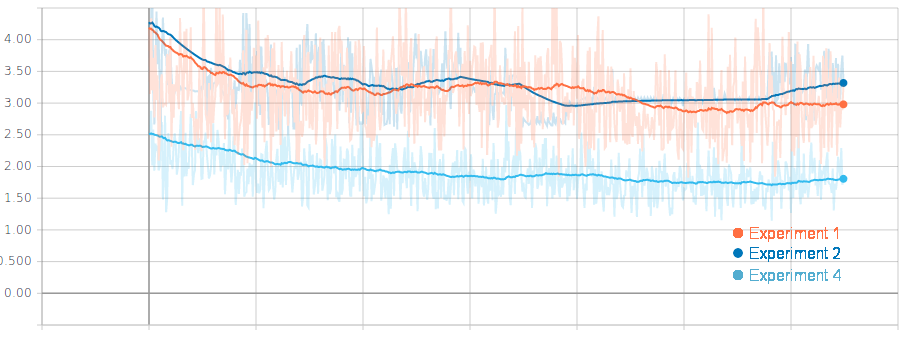
\includegraphics[width=0.95\linewidth]{images/evaluation/slm-k-losses-2.png}
	\label{fig:loss650epochs2}
\end{figure}

\subsection{OnlyStockLearningModel results}
In figure \ref{fig:OSLM_k-accuracy} you can see the accuracy of the four experiments described in table \ref{tbl:experiments}. The loss can be seen in figure \ref{fig:OSLM_k-loss}. The models without using dropout performed best. This seems to be reasonable because if the dropout drops the only input, like in the other two experiments, the model can not use any data for learning. The model with the biggest hidden size (experiment 3) is not performing better than the other models and therefore it does not make sense to increase the hidden size. The model of experiment 4 has the lowest learning rate and therefore can find a better minimum than the other three models.\\
\begin{figure}[tb]
	\caption{A Graph depicting the mean accuracy of the OnlyStockLearningModel over 650 epochs of the k fold cross validation with $k=10$. The orange line shows the accuracy during training for experiment 1. Its mean accuracy is about $49\%$. The red line showing experiment 2 has about the same mean accuracy. The light blue graph is presenting the results of the third experiment. It has a mean accuracy of about $52\%$. The best result is of the forth experiment with about $55\%$ accuracy.}
	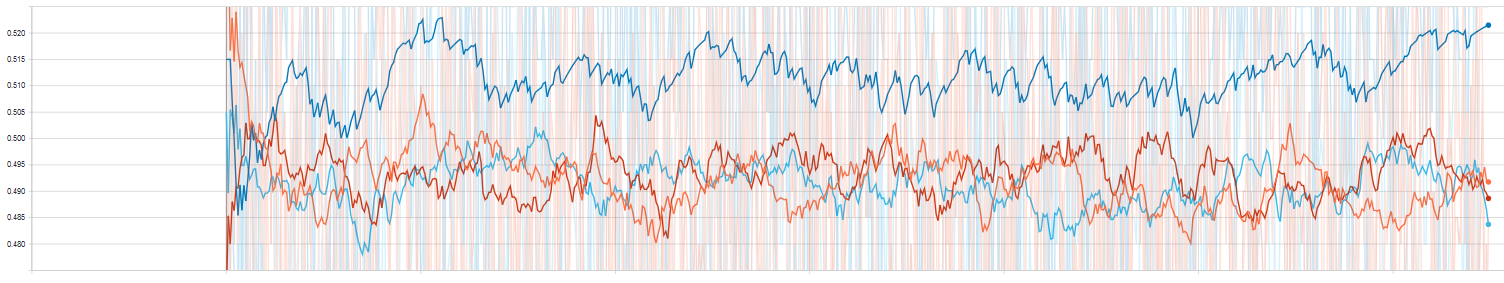
\includegraphics[width=0.95\linewidth]{images/OSLM_k-accuracy.PNG}
	\label{fig:OSLM_k-accuracy}
\end{figure}
\begin{figure}[tb]
	\caption{A Graph depicting the mean loss of the OnlyStockLearningModel over 650 epochs of the k fold cross validation with $k=10$. The orange line depicts the loss of the first experiment. It has nearly the same mean loss of about $4.7$ as the dark (experiment 2) and light (experiment 4) blue lines. The loss of experiment 4 is shown in the red line. Its mean value is about $24.6$.}
	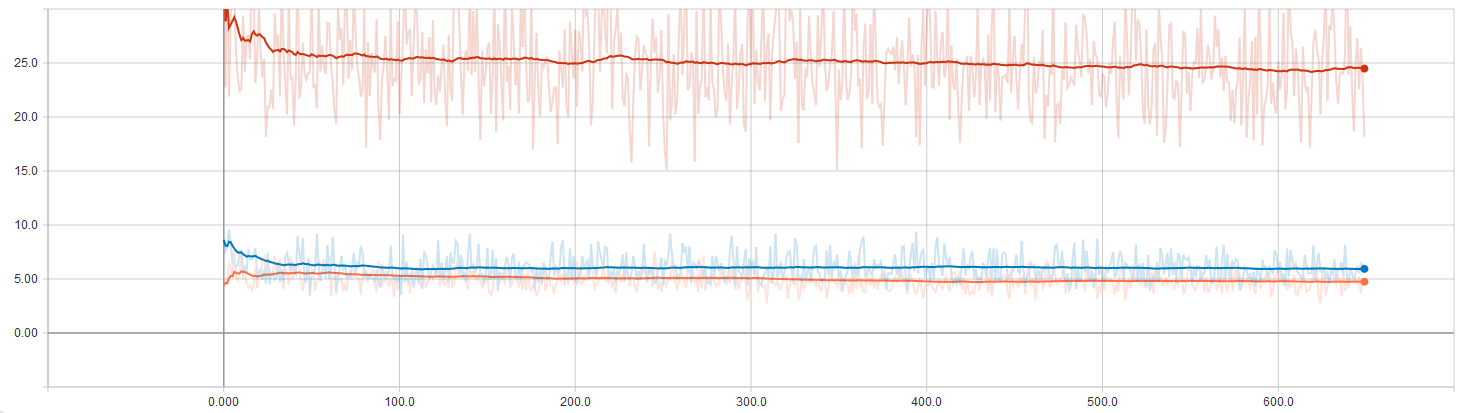
\includegraphics[width=0.95\linewidth]{images/OSLM_k-loss.PNG}
	\label{fig:OSLM_k-loss}
\end{figure}
In the following listing you can see how the models performed on data not seen during training. The test dataset contains only 16 entries, so the results have to be watched carefully.
\begin{itemize}
	\item Experiment 1: $53.63\%$ accuracy
	\item Experiment 2: $50\%$ accuracy
	\item Experiment 3: $46.88\%$ accuracy
	\item Experiment 4: $50\%$ accuracy
\end{itemize}
The models without using dropout have a lower accuracy than they reached during training. The model of the first experiment is even better on this test data than it was during training. Whereas the third model is performing bad on unseen data. All four models do not have an accuracy which is good enough to make me belief that they can predict the trend of a stock better than an financial expert could do.


\subsection{Comparison of model results}
\label{subsec:compmodelresults}	
TODO


\section{Conclusion}
\label{sec:ausblick}
In this paper 
+ results of the project to predict rising or falling stocks using deep learning methods are presented
+ the basic framework for
	- retrieving the google trends data
	- preprocess the data
	- learning models
	implemented
+ simple learning model, which uses a lstm, achieved an accuracy of 53\% , just above simple guessing 
+ after ca. 150 epochs with k fold cross validation (k=10) and dropout the accuracy reached its max - longer training was contra productive 

+ simplified approach therefore does not encourage further research of predicting stocks based on google trend data
+ however as only the lstm, and only a single cell, was used, other models and model combinations could yield better results
+ as the architecture for this project was implemented flexible for future extensions, it could serve as a starting point / core for this future research. for example, another model could be derived from the abstract class and used instead

simplified approach reached xx\% of accuracy, therefore it would be worthwhile to enhance the current model by predicting ranges of values, e.g. 50 up or down etc.
as described in \ref{sec:architecture}, only minor changes would only be necessary
\begin{itemize}
	\item summarize the results (implementation? evaluation results?) 
	\item does it work? why? why not? 
	\item how could the current solution be improved? 
	\item possible further research? 
	\item how fast must it be. Finance is fast changing market
\end{itemize}


\bibliography{mybib}{}
\end{document}
